% dieWolke: first SEN12MS-CR (spring) evaluation, IEEE conference format (IEEEtran).
% Written for readers outside the field: every term is explained where it first appears.
% Numbers are copied from RESULTS.md and the evaluation reports (kaggle_logs/eval/*/report.md).
% Build: pdflatex dieWolke_ieee.tex (twice), or upload to Overleaf; IEEEtran.cls ships with TeX Live.
\documentclass[conference]{IEEEtran}
\usepackage{cite}
\usepackage{amsmath,amssymb,amsfonts}
\usepackage{graphicx}
\usepackage{textcomp}
\usepackage{xcolor}
\usepackage{booktabs}
\usepackage{pgfplots}
\pgfplotsset{compat=1.17}
\usepackage[hidelinks]{hyperref}

\newcommand{\best}[1]{\textbf{#1}}

\begin{document}

\title{Seeing Through Clouds: Using Radar to Rebuild Cloud-Covered Sentinel-2 Satellite Images}

% TODO: replace with the real author names and affiliations
\author{\IEEEauthorblockN{Author One}
\IEEEauthorblockA{\textit{Department} \\
\textit{Institution}\\
City, Country \\
email@example.com}
\and
\IEEEauthorblockN{Author Two}
\IEEEauthorblockA{\textit{Department} \\
\textit{Institution}\\
City, Country \\
email@example.com}
}

\maketitle

\begin{abstract}
Satellite photos of farmland are often useless because clouds cover the ground, and this happens
most during the monsoon, exactly when farmers and planners need the data. Radar satellites can
see through clouds, but radar images do not look like photos. We built a deep learning model,
called dieWolke, that takes a cloudy Sentinel-2 image together with a Sentinel-1 radar image of
the same place and predicts what the ground looks like without clouds, in all 13 spectral bands
that Sentinel-2 records. On top of a standard design we tested four ideas: processing related
bands in separate branches, checking a vegetation index (NDVI) during training, letting the model
say how confident it is in each pixel, and finding the clouds first in a separate step. We
trained on a small dataset (2,434 image patches) and tested on 1,500 patches from places the
model had never seen. Our model comes within 0.5--0.7\,dB of two published models that were
trained on far more data, and beats a classical machine-learning method by more than 2\,dB.
Finding the clouds first is clearly the right choice (1.1\,dB better than skipping that step),
and the confidence map is genuinely useful: ignoring the least confident half of the pixels cuts
vegetation-index errors by 26\,\%. The vegetation-index check helps a little, and splitting the
bands into branches did not help with this amount of data.
\end{abstract}

\begin{IEEEkeywords}
cloud removal, satellite imagery, radar, Sentinel-1, Sentinel-2, deep learning, agriculture
\end{IEEEkeywords}

\section{Introduction}
The European Sentinel-2 satellites photograph the whole Earth every few days. Unlike a normal
camera, which records three colours, they record 13 \emph{bands}: the visible colours plus
several invisible ones in the near- and short-wave infrared. Those invisible bands are what make
the images so useful for farming, because healthy plants reflect strongly in the near infrared
and wet soil looks different from dry soil in the short-wave infrared. A simple number computed
from the red and near-infrared bands, the \emph{NDVI} (Normalised Difference Vegetation Index),
is the standard way to measure how green and healthy crops are.

The problem is clouds. In India's Kharif season (July to October), the main monsoon growing
season, most Sentinel-2 images of farmland are partly or completely cloudy. The data is missing
exactly when it matters most.

The Sentinel-1 satellites carry a radar instead of a camera. Radar sends out its own microwave
signal, which passes through clouds, so Sentinel-1 always sees the ground. Radar images, however,
show surface texture and moisture rather than colour, so they cannot simply replace the photo.

The idea behind this project, and behind earlier work such as DSen2-CR~\cite{meraner2020dsen2cr},
GLF-CR~\cite{xu2022glfcr} and UnCRtainTS~\cite{ebel2023uncrtaints}, is to give a neural network
both images: the cloudy photo shows what the clear parts look like, and the radar gives clues
about what is hidden under the clouds. The network learns to fill in the gaps.

\textbf{What we add.} Combining radar and optical images is not new, and neither is the type of
model we use (a so-called diffusion bridge~\cite{hu2025dbcr}). What we contribute are four
additions aimed at agricultural use, each tested carefully on its own:
\begin{itemize}
\item \textbf{Band groups (C1):} the visible, the plant-sensitive (red-edge and near infrared) and
the moisture-sensitive (short-wave infrared) bands are handled by separate branches of the
network, because they behave differently.
\item \textbf{Vegetation check (C2):} during training, the model is also penalised when the NDVI of
its output is wrong, not only when the pixels are wrong.
\item \textbf{Confidence map (C3):} the model outputs, for every pixel, how sure it is of its own
answer, so users know which parts to trust.
\item \textbf{Clouds first (C5):} a small separate network first finds the clouds and their
shadows, and only then does the main network fill them in.
\end{itemize}
A fifth part of the project (C4), a test set built from real Indian Kharif fields, is in progress
and not covered here.

\textbf{How we test.} All versions of our model share the same design, training time and data, so
when we switch one idea off, any change in the results comes from that idea alone. We also ran the
published UnCRtainTS and GLF-CR models, using their authors' own trained weights, through exactly
the same test code. Ideas that did not work are reported as such.

\section{Related Work}
\textbf{Radar plus optical.} DSen2-CR~\cite{meraner2020dsen2cr} was one of the first deep networks
to combine Sentinel-1 radar with cloudy Sentinel-2 images, together with the SEN12MS-CR dataset of
matching radar, cloudy and clear images from around the world~\cite{ebel2021sen12mscr}. GLF-CR
\cite{xu2022glfcr} improved how the two kinds of image are combined, and UnCRtainTS
\cite{ebel2023uncrtaints} added an estimate of how uncertain each prediction is.

\textbf{Diffusion models.} Diffusion models are the family behind modern AI image generators. A
\emph{diffusion bridge} is a variant that learns to turn one image into another, here a cloudy
image into a clear one~\cite{li2023bbdm}. DB-CR~\cite{hu2025dbcr} applied this to cloud removal
with radar, and CloudBreaker~\cite{ahmed2025cloudbreaker} produces four optical bands from radar
alone.

\textbf{Classical methods.} Gupta and Verma~\cite{gupta2026cloudfree} filled cloudy Sentinel-2
pixels in India with tree-based machine learning before classifying crops. Our XGBoost
comparison~\cite{chen2016xgboost} follows the same spirit, but it is our own implementation,
not theirs.

\section{How the Model Works}

\subsection{Inputs and outputs}
For each location the model receives three things: the cloudy Sentinel-2 image (13 bands), a
Sentinel-1 radar image (two channels, called VV and VH), and a \emph{cloud mask}, a black-and-white
map of which pixels are covered by cloud or cloud shadow. It outputs the 13-band cloud-free image
and, optionally, a confidence map. All images are 256$\times$256 pixels, or 2.56\,km by 2.56\,km
on the ground. Pixel values are scaled to the range 0 to 1.

\subsection{The bridge between cloudy and clear}
Picture a slider with the cloudy image at one end and the clear image at the other. Positions in
between are a blend of the two plus a little random noise. During training, the network is shown
points along this slider and has to work out the clear end. Formally, the point at position $t$
(0 = clear, 1 = cloudy) is
\begin{equation}
x_t = (1-t)\,x_{\mathrm{clear}} + t\,x_{\mathrm{cloudy}} + \sigma\sqrt{t(1-t)}\,\epsilon,
\end{equation}
where $\epsilon$ is random noise and $\sigma = 0.5$ sets how much noise is added. At $t = 1$ the
point is exactly the cloudy image, with no noise. When the model is used, it starts there and
jumps to the clear end in a single step, which makes it fast. All results in this paper use this
one-step mode. During training, a quarter of the examples are taken at exactly $t = 1$ so that
the model gets plenty of practice at this one-step jump.

\subsection{The network}
The main network is a U-Net, a standard design for image tasks that first shrinks the image to
understand the overall scene and then expands it back to full size to produce detailed output.
It has four levels of detail. A separate radar branch turns the radar image into features at
every level, and \emph{attention} layers at the coarser levels let the optical part of the network
look up the relevant radar information. Pixels that are not cloudy are copied straight from the
input, so the network only has to fill in what is hidden. Training minimises the average
difference between the predicted and the true clear image (an L1 loss), plus the extra terms
described below.

\subsection{C1: Band groups}
In the full model the input layer, every attention layer and the output layer are split into
three branches: visible (bands B01--B04), red-edge and near infrared (B05--B08, B8A, B09) and
short-wave infrared (B10--B12). Each branch has its own weights and its own view of the radar
features, and the branches share a short summary with each other. The comparison version replaces
the branches with a single shared layer of about the same size.

\subsection{C2: Vegetation check}
The loss gets an extra term: the difference between the NDVI of the predicted image and the NDVI
of the true image, with weight 0.1. NDVI is a ratio, and on very dark pixels (water, shadow,
missing data) its value jumps wildly; in our first runs this made training break down. We
therefore leave out pixels where the red and near-infrared bands are both very dark.

\subsection{C3: Confidence map}
For each pixel and band, the model also predicts a spread $b$: a small $b$ means ``I am sure'',
a large $b$ means ``I might be far off''. It learns this by being rewarded when large errors come
with a large spread and small errors with a small spread~\cite{kendall2017uncertainties}. This
extra task is kept separate from the main prediction, so switching it on does not change what the
main image is trained on. After training, the spreads are rescaled slightly so that they match the
real errors on held-out data (\emph{calibration}~\cite{guo2017calibration}).

\subsection{C5: Finding the clouds first}
On real cloudy images nobody knows the exact cloud outline, so we estimate it with a standard
cloud detector, s2cloudless~\cite{zupanc2017s2cloudless}, plus a simple rule for shadows
\cite{zhai2018cloudshadow}. To get images where the right answer is known exactly, we also create
\emph{synthetic} cloudy images: a real cloud is cut out of one image and pasted, with its shadow,
onto a clear image of another place. The cloud-finding network (a small U-Net) is trained on these
synthetic images and finds the cloud-and-shadow area with an overlap (IoU) of 0.964 with the truth
on validation data. For comparison, an \emph{end-to-end} version gets no cloud mask at all and has
to figure out the clouds by itself while reconstructing.

\section{Experiments}

\subsection{Data}
We use SEN12MS-CR~\cite{ebel2021sen12mscr}, a public dataset of matching radar, cloudy and clear
images. To keep the first experiments small and fast, we use only its spring part. From the
training areas we took a random sample of 2,500 patches; after removing pairs whose ``clear''
image was itself more than 5\,\% cloudy, 2,434 remained for training. We use 300 patches for
validation (choosing the best checkpoint) and 1,500 patches from five test areas that the model
never sees during training. Because we use only spring data, our numbers should not be compared
directly with papers that use all four seasons, such as DB-CR~\cite{hu2025dbcr}.

\subsection{Training}
Each model was trained on free NVIDIA T4 graphics cards on Kaggle, with batches of 8 random
128$\times$128 crops (flipped and rotated for variety), the AdamW optimiser with a learning rate
of $2\times10^{-4}$ that slowly decreases, and a smoothed average of the weights. The full model and
the comparison model trained for 40,000 steps; the experiments that switch one idea off trained
for 20,000 steps each, against a 20,000-step copy of the full model. Each version was trained once.

\subsection{What we compare}
\begin{itemize}
\item \textbf{Ours, full:} with C1, C2 and C3 switched on.
\item \textbf{Ours, matched:} the identical model with C1, C2 and C3 switched off. This is the fair
test of whether our additions help.
\item \textbf{UnCRtainTS and GLF-CR:} published models, run with their authors' weights. They were
trained on all four seasons of SEN12MS-CR, far more data than ours. As a sanity check, UnCRtainTS
scores 28.83\,dB on our spring test set, close to the 28.90\,dB its authors report on the full test
set~\cite{ebel2023uncrtaints}, which tells us we are feeding it data correctly.
\item \textbf{XGBoost:} a classical machine-learning method that, for each image, learns from the
clear pixels how radar relates to each band, then fills in the cloudy pixels.
\item \textbf{Cloudy input:} doing nothing, as a floor.
\end{itemize}

\subsection{How we score}
\begin{itemize}
\item \textbf{PSNR} (peak signal-to-noise ratio, in dB): how close the output is to the true
image; higher is better, and in this field a gain of 1\,dB is considered substantial.
\item \textbf{SSIM} (0 to 1): how well shapes and textures match; higher is better.
\item \textbf{SAM} (degrees): how well the ``spectral signature'' of each pixel, its pattern across
the 13 bands, matches; lower is better.
\item \textbf{NDVI error} (RMSE): how far off the vegetation index is; lower is better.
\end{itemize}
All are computed on all 13 bands for each test image and then averaged. ``Cloud'' versions use
only the pixels that were under cloud. When we say one model is better than another, we give a
95\,\% confidence interval in square brackets, computed by resampling the test images; if the
interval includes zero, the difference could be chance.

\section{Results}

\subsection{Main comparison}
Table~\ref{tab:main} shows the results on real clouds. Every deep model improves the image by
about 10\,dB over doing nothing and beats XGBoost by more than 2\,dB. Our full model is slightly
behind our matched model (0.20\,dB [0.14, 0.27]). The published models are ahead of ours by
0.46--0.71\,dB, which is not surprising given that they learned from many times more data. GLF-CR
has clearly the most accurate vegetation index.

\begin{table}[t]
\centering
\caption{Real clouds, 1,500 test patches. Higher PSNR and SSIM are better; lower SAM and NDVI
error are better. Our models learned from 2,434 spring patches; the published models from all of
SEN12MS-CR.}
\label{tab:main}
\setlength{\tabcolsep}{4pt}
\begin{tabular}{lcccc}
\toprule
Method & PSNR & SSIM & SAM & NDVI error \\
\midrule
Cloudy input (do nothing) & 18.62 & 0.676 & 13.82 & 0.269 \\
XGBoost (classical) & 25.98 & 0.803 & 9.54 & 0.167 \\
Ours, full & 28.12 & 0.866 & 8.40 & 0.153 \\
Ours, matched & 28.32 & 0.870 & 8.32 & 0.152 \\
UnCRtainTS (published) & \best{28.83} & 0.882 & 8.00 & 0.145 \\
GLF-CR (published) & 28.59 & \best{0.887} & \best{7.79} & \best{0.129} \\
\bottomrule
\end{tabular}
\end{table}

\subsection{Where the difference comes from}
Fig.~\ref{fig:cloudfrac} splits the test images by how cloudy they are, and this tells an
interesting story. When an image is almost completely covered (90\,\% cloud or more, which is
almost half the test set), the model has nothing to go on except the radar, and all four deep
models score within 0.2\,dB of each other. Our full model is level with our matched model and with
GLF-CR there, and only 0.20\,dB behind UnCRtainTS.

The published models pull ahead on \emph{partly} cloudy images, by 0.8--1.2\,dB. To do well on
those, a model has to combine the visible pixels with the radar, and cope with the fact that the
cloudy and the clear photo were taken on different days. That is the kind of skill that comes from
seeing many examples, so more training data should help us most here.

The ranking also changes from place to place. In one test area both of our models beat
UnCRtainTS, and in the cloudiest area our full model beats both our matched model and GLF-CR.
With only five test areas, the overall ranking is less certain than the confidence intervals
suggest.

\begin{figure}[t]
\centering
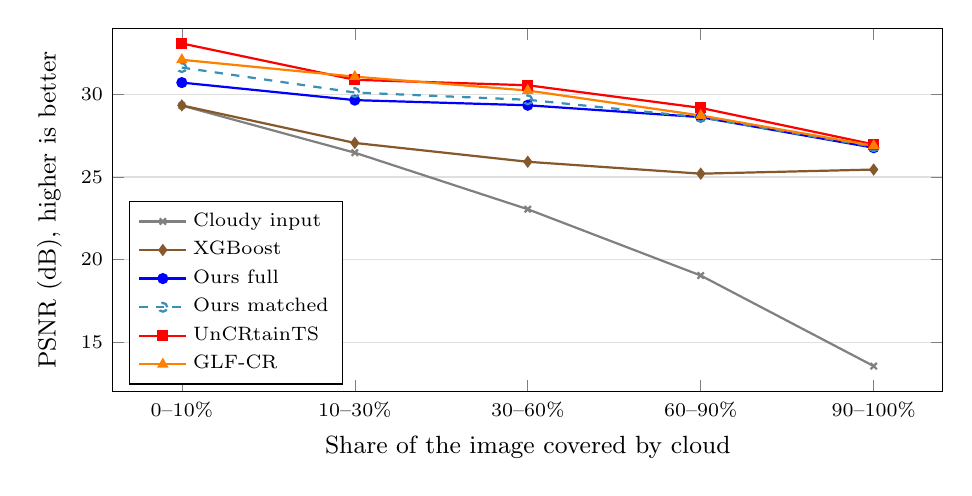
\begin{tikzpicture}
\begin{axis}[
  width=\columnwidth, height=6.2cm,
  symbolic x coords={0--10\%,10--30\%,30--60\%,60--90\%,90--100\%},
  xtick=data, xlabel={Share of the image covered by cloud}, ylabel={PSNR (dB), higher is better},
  ymin=12, ymax=34, ymajorgrids, grid style={gray!25},
  legend style={font=\scriptsize, at={(0.02,0.02)}, anchor=south west, cells={anchor=west}},
  tick label style={font=\scriptsize}, label style={font=\small},
  every axis plot/.append style={thick, mark size=1.6pt},
]
\addplot[gray, mark=x] coordinates {(0--10\%,29.32) (10--30\%,26.47) (30--60\%,23.05) (60--90\%,19.04) (90--100\%,13.56)};
\addplot[brown!70!black, mark=diamond*] coordinates {(0--10\%,29.33) (10--30\%,27.06) (30--60\%,25.92) (60--90\%,25.20) (90--100\%,25.45)};
\addplot[blue, mark=*] coordinates {(0--10\%,30.71) (10--30\%,29.65) (30--60\%,29.34) (60--90\%,28.62) (90--100\%,26.77)};
\addplot[cyan!70!black, dashed, mark=o] coordinates {(0--10\%,31.62) (10--30\%,30.11) (30--60\%,29.67) (60--90\%,28.61) (90--100\%,26.83)};
\addplot[red, mark=square*] coordinates {(0--10\%,33.08) (10--30\%,30.88) (30--60\%,30.55) (60--90\%,29.18) (90--100\%,26.97)};
\addplot[orange, mark=triangle*] coordinates {(0--10\%,32.09) (10--30\%,31.07) (30--60\%,30.23) (60--90\%,28.72) (90--100\%,26.89)};
\legend{Cloudy input, XGBoost, Ours full, Ours matched, UnCRtainTS, GLF-CR}
\end{axis}
\end{tikzpicture}
\caption{Quality versus cloud cover on real clouds (139, 148, 196, 299 and 718 test patches per
group). Under near-total cloud the deep models are almost equal; the published models lead on
partly cloudy images.}
\label{fig:cloudfrac}
\end{figure}

\subsection{Synthetic clouds}
With pasted clouds we know the exact truth underneath and the exact cloud outline
(Table~\ref{tab:synth}). Here the picture flips: our full model is 0.20\,dB [0.12, 0.28]
\emph{ahead} of the matched model, with better spectral and vegetation accuracy, although the
matched model keeps a slightly better SSIM. So whether our additions help depends on the type of
cloud, and neither version is better across the board.

\begin{table}[t]
\centering
\caption{Synthetic clouds (real clouds pasted onto clear images, so the truth is known exactly).}
\label{tab:synth}
\setlength{\tabcolsep}{4pt}
\begin{tabular}{lcccc}
\toprule
Method & PSNR & SSIM & SAM & NDVI error \\
\midrule
Cloudy input & 19.51 & 0.689 & 8.81 & 0.226 \\
Ours, full & \best{29.08} & 0.870 & \best{7.49} & \best{0.148} \\
Ours, matched & 28.88 & \best{0.876} & 7.62 & 0.151 \\
\bottomrule
\end{tabular}
\end{table}

\subsection{Testing each idea on its own}
Table~\ref{tab:abl} switches off one idea at a time. Surprisingly, switching off any of them makes
the overall image slightly \emph{better}: by 0.36\,dB without band groups, 0.16\,dB without the
vegetation check and 0.15\,dB without the confidence map. The vegetation check does do its own job:
without it, the NDVI error goes up by about 3.5\,\% (0.0053 [0.0038, 0.0067]). The band groups,
on the other hand, do not even improve the bands they were designed for; the red-edge,
near-infrared and short-wave infrared errors are the same or lower without them.

\begin{table}[t]
\centering
\caption{Switching off one idea at a time (real clouds, 20,000 training steps each). The last
column is the change in PSNR compared with the full model, with its confidence interval.}
\label{tab:abl}
\setlength{\tabcolsep}{3pt}
\begin{tabular}{lccc}
\toprule
Version & PSNR & NDVI error & Change in PSNR \\
\midrule
Full (all ideas on) & 27.84 & 0.152 & --- \\
Without band groups & 28.20 & 0.153 & $+0.36$ [0.29, 0.44] \\
Without vegetation check & 28.00 & 0.157 & $+0.16$ [0.11, 0.20] \\
Without confidence map & 27.99 & 0.149 & $+0.15$ [0.09, 0.21] \\
\bottomrule
\end{tabular}
\end{table}

\subsection{Finding the clouds first}
This is our clearest result (Table~\ref{tab:c5}). Without a cloud mask, the model is 1.1\,dB
worse overall [0.98, 1.20], 1.4\,dB worse under the clouds, and has a much lower SSIM (0.78 versus
0.86). It is better on only about a quarter of the images. Just as important, the masks from our
own cloud-finding network work as well as the exact masks, so the two-step design costs nothing.

\begin{table}[t]
\centering
\caption{Finding clouds first versus not using a mask (synthetic clouds).}
\label{tab:c5}
\setlength{\tabcolsep}{4pt}
\begin{tabular}{lccc}
\toprule
Version (20,000 steps) & PSNR & SSIM & PSNR under cloud \\
\midrule
With the exact cloud mask & 28.75 & 0.863 & 27.56 \\
With our cloud finder's mask & 28.76 & 0.864 & 27.58 \\
No mask at all & 27.66 & 0.784 & 26.20 \\
\bottomrule
\end{tabular}
\end{table}

\subsection{The confidence map}
The confidence map is useful. Pixels where the model says it is unsure really do have larger
errors (rank correlation 0.43 on real clouds, 0.55 on synthetic ones), and after calibration its
stated confidence matches reality more closely (calibration error 0.055, down from 0.085). The
practical test is in Table~\ref{tab:unc}: if we throw away the pixels the model is least sure
about, the vegetation index of the remaining pixels gets steadily more accurate, and keeping the
most confident half cuts the NDVI error by 26\,\%. One caution: the calibration learned on real
clouds made the synthetic-cloud calibration worse, so it does not carry over between cloud types.

\begin{table}[t]
\centering
\caption{Keeping only the pixels the model is most confident about (real clouds).}
\label{tab:unc}
\begin{tabular}{lcccc}
\toprule
Share of pixels kept & 100\,\% & 90\,\% & 75\,\% & 50\,\% \\
\midrule
NDVI error & 0.182 & 0.171 & 0.158 & 0.134 \\
\bottomrule
\end{tabular}
\end{table}

\section{Discussion and Limitations}
\textbf{More data is the obvious next step.} Our models learned from 2,434 patches; the published
models from the whole dataset. Their advantage is concentrated on partly cloudy images, which is
where more examples should help most. We are now retraining on a much larger part of the spring
training data (which has 24,378 patches in total) to find out whether the gap is about data or
about design.

\textbf{Band groups did not work, for now.} Splitting the bands into branches made results slightly
worse and did not help the targeted bands. It may need more data to pay off, or it may simply not
be a useful idea for this task; we do not claim it as a contribution based on these results.

\textbf{Things to keep in mind.} Each version was trained only once, so small differences of a few
tenths of a dB between our own versions might change with another training run. The test set
comes from only five areas. The cloud outlines on real images are estimates. And all results are
for spring images only.

\section{Conclusion}
A radar-guided model can rebuild cloud-covered Sentinel-2 images in all 13 bands well, even when
trained on a small dataset: it comes within 0.5--0.7\,dB of published models trained on far more
data and is more than 2\,dB better than a classical method. Two of our ideas clearly earn their
place: finding the clouds first, and giving a confidence map that tells users which pixels to
trust, which makes the vegetation index 26\,\% more accurate when the unsure half is set aside.
The vegetation check is a small trade-off, and the band groups did not help at this scale. Next,
we will train on more data, repeat the key runs, and test the model on real Indian Kharif fields
with a crop classification task.

\begin{thebibliography}{00}
\bibitem{ebel2021sen12mscr} P. Ebel, A. Meraner, M. Schmitt, and X. X. Zhu, ``Multisensor data
fusion for cloud removal in global and all-season Sentinel-2 imagery,'' \textit{IEEE Trans.
Geosci. Remote Sens.}, vol.~59, no.~7, pp.~5866--5878, 2021.
\bibitem{meraner2020dsen2cr} A. Meraner, P. Ebel, X. X. Zhu, and M. Schmitt, ``Cloud removal in
Sentinel-2 imagery using a deep residual neural network and SAR-optical data fusion,''
\textit{ISPRS J. Photogramm. Remote Sens.}, vol.~166, pp.~333--346, 2020.
\bibitem{xu2022glfcr} F. Xu, Y. Shi, P. Ebel, L. Yu, G.-S. Xia, W. Yang, and X. X. Zhu, ``GLF-CR:
SAR-enhanced cloud removal with global--local fusion,'' \textit{ISPRS J. Photogramm. Remote
Sens.}, vol.~192, pp.~268--278, 2022.
\bibitem{ebel2023uncrtaints} P. Ebel, V. S. F. Garnot, M. Schmitt, J. D. Wegner, and X. X. Zhu,
``UnCRtainTS: Uncertainty quantification for cloud removal in optical satellite time series,'' in
\textit{Proc. IEEE/CVF Conf. Comput. Vis. Pattern Recognit. Workshops (CVPRW)}, 2023;
arXiv:2304.05464.
\bibitem{hu2025dbcr} Y. Hu, S. Lohit, U. S. Kamilov, and T. K. Marks, ``Multimodal diffusion
bridge with attention-based SAR fusion for satellite image cloud removal,'' arXiv:2504.03607,
2025.
\bibitem{li2023bbdm} B. Li, K. Xue, B. Liu, and Y.-K. Lai, ``BBDM: Image-to-image translation with
Brownian bridge diffusion models,'' in \textit{Proc. IEEE/CVF Conf. Comput. Vis. Pattern
Recognit. (CVPR)}, 2023, pp.~1952--1961.
\bibitem{ahmed2025cloudbreaker} S. S. Ahmed, S. Nowreen, and M. S. Rahman, ``CloudBreaker:
Breaking the cloud covers of Sentinel-2 images using multi-stage trained conditional flow
matching on Sentinel-1,'' arXiv:2508.03608, 2025.
\bibitem{gupta2026cloudfree} S. Gupta and P. A. Verma, ``Generating cloud-free Sentinel-2 images
for enhanced in-season crop type classification: A case study,'' \textit{Remote Sens. Earth Syst.
Sci.}, 2026, doi:10.1007/s41976-025-00254-z.
\bibitem{chen2016xgboost} T. Chen and C. Guestrin, ``XGBoost: A scalable tree boosting system,'' in
\textit{Proc. 22nd ACM SIGKDD Int. Conf. Knowl. Discov. Data Min.}, 2016, pp.~785--794.
\bibitem{kendall2017uncertainties} A. Kendall and Y. Gal, ``What uncertainties do we need in
Bayesian deep learning for computer vision?'' in \textit{Adv. Neural Inf. Process. Syst.
(NeurIPS)}, 2017.
\bibitem{guo2017calibration} C. Guo, G. Pleiss, Y. Sun, and K. Q. Weinberger, ``On calibration of
modern neural networks,'' in \textit{Proc. Int. Conf. Mach. Learn. (ICML)}, 2017.
\bibitem{zupanc2017s2cloudless} A. Zupanc, ``Improving cloud detection with machine learning,''
Sentinel Hub blog, 2017. [Online]. Available: https://medium.com/sentinel-hub
\bibitem{zhai2018cloudshadow} H. Zhai, H. Zhang, L. Zhang, and P. Li, ``Cloud/shadow detection
based on spectral indices for multi/hyperspectral optical remote sensing imagery,'' \textit{ISPRS
J. Photogramm. Remote Sens.}, vol.~144, pp.~235--253, 2018.
\end{thebibliography}

\end{document}
